\documentclass[11pt]{article}


% Lengths ----------------------------------------------------------------------

% save parindent to a new length, originalparindent
\newlength{\originalparindent}
\setlength{\originalparindent}{\parindent}

% set parskip to bigskipamount for space between paragraphs
\setlength{\parskip}{\bigskipamount}

% set parindent to 0pt for disabling paragraph indentation
\setlength{\parindent}{0pt}


% Packages ---------------------------------------------------------------------

% geometry package for setting page
% size, and for refining page margins
\usepackage[a4paper, hscale=0.85, vscale=0.85]{geometry}

% Set font encoding
\usepackage[T1]{fontenc}

% url package for handlink hyperlinks
\usepackage{url}

% hyperref package for handling in-document links and styling links
\usepackage{hyperref}

% fontspec package to load custom fonts
\usepackage{fontspec}

% xcolor package for
\usepackage[table]{xcolor}

% secdot package for adding dot after section numbers
\usepackage{secdot}

% ulem package for enabling strikethrough
\usepackage[normalem]{ulem}

% tocloft package for disabling
% bold font in the table of contents
\usepackage{tocloft}

% titletoc package for adding a dot after
% section numbers in the table of contents
\usepackage[dotinlabels]{titletoc}

% setspace package for altering linespread in tables
\usepackage{setspace}

% float package for placing tables
% and figure at exact position
\usepackage{float}

% caption package
% for caption styling
\usepackage{caption}

% colortbl package for colored tables
\usepackage{colortbl}

% tikz package for inline code
% styling, and horizontal rules
\usepackage{tikz}

% verbatim package for verbatim
% environment in code block environments
\usepackage{verbatim}

% mdframed environment for custom
% code blocks and custom quotes
% (common options for all mdframed based
% environments are set at package loading)
\usepackage[framemethod=tikz,%
    innerleftmargin=0.5\originalparindent,%
    innerrightmargin=0.5\originalparindent,%
    skipabove=0.4\baselineskip,%
    skipbelow=0.4\baselineskip,%
    innertopmargin=0.4\baselineskip,%
    innerbottommargin=0.4\baselineskip]{mdframed}

% tabu package for
% easier tabular styling
\usepackage{tabu}


% Package Setups ---------------------------------------------------------------

% setup for hyperref package:
%   enabled pdf bookmarks,
%   setting link styles
\hypersetup{bookmarks=true,%
    bookmarksnumbered=true,%
    pdfencoding=unicode,%
    colorlinks=true,%
    pdfborder={0 0 0},%
    linkcolor=black,%
    menucolor=black,%
    citecolor=mdhyperlinkcolor,%
    urlcolor=mdhyperlinkcolor,%
    filecolor=mdhyperlinkcolor}

% setup for tikz package:
%   load library for fancy hrlues
\usetikzlibrary{decorations.pathreplacing}

% setup url package:
%   set url font to sans serif instead of teletype
\urlstyle{sf}

% Font settings ----------------------------------------------------------------

% set document default font to Source Sans Pro and its variants

\setmainfont[Mapping=tex-text,%
    ItalicFont=Source Sans Pro Light Italic,%
    BoldFont=Source Sans Pro,%
    BoldItalicFont=Source Sans Pro Italic]{Source Sans Pro Light}

% set sans serif font to Source Sans Pro and its variants (just in case)
\setsansfont[Mapping=tex-text,%
    ItalicFont=Source Sans Pro Light Italic,%
    BoldFont=Source Sans Pro,%
    BoldItalicFont=Source Sans Pro Italic]{Source Sans Pro Light}

% set monospace font to Source Code Pro and its variants
\setmonofont[Mapping=tex-text,%
    ItalicFont=Source Code Pro ExtraLight,%
    BoldFont=Source Code Pro]{Source Code Pro Light}

% Color definitions ------------------------------------------------------------

\definecolor{mdfancyhlinecolor}{HTML}{CCCCCC}
\definecolor{mdsimplehlinecolor}{HTML}{DDDDDD}
\definecolor{mdhyperlinkcolor}{HTML}{4183C4}
\definecolor{mdinlinecodeboxbackgroundcolor}{HTML}{F8F8F8}
\definecolor{mdinlinecodeboxframecolor}{HTML}{DDDDDD}
\definecolor{mdblockquotelinecolor}{HTML}{DDDDDD}
\definecolor{mdalternatingtablerowcolor}{HTML}{F8F8F8}
\definecolor{mdtableframecolor}{HTML}{DDDDDD}
\definecolor{mdimgboxcolor}{HTML}{DDDDDD}


% Styling table of contents ----------------------------------------------------

% set dot fill style
\renewcommand{\cftsecdotsep}{\cftdotsep}
\renewcommand{\cftsubsecdotsep}{\cftdotsep}
\renewcommand{\cftsubsubsecdotsep}{\cftdotsep}
\renewcommand{\cftparadotsep}{\cftdotsep}
\renewcommand{\cftsubparadotsep}{\cftdotsep}
\renewcommand{\cftsecleader}{\cftdotfill{\cftsecdotsep}}
\renewcommand{\cftsubsecleader}{\cftdotfill{\cftsubsecdotsep}}
\renewcommand{\cftsubsubsecleader}{\cftdotfill{\cftsubsubsecdotsep}}
\renewcommand{\cftparaleader}{\cftdotfill{\cftparadotsep}}
\renewcommand{\cftsubparaleader}{\cftdotfill{\cftsubparadotsep}}

% set section font style
\renewcommand\cftsecfont{\normalfont}
\renewcommand\cftsecpagefont{\normalfont}

% set indentation of toc entries
\newlength{\mycftsecindent}
\newlength{\mycftsubsecindent}
\newlength{\mycftsubsubsecindent}
\newlength{\mycftparaindent}
\newlength{\mycftsubparaindent}
\setlength{\mycftsecindent}{0.5\cftsecindent}
\setlength{\mycftsubsecindent}{0.5\cftsubsecindent}
\setlength{\mycftsubsubsecindent}{0.5\cftsubsubsecindent}
\setlength{\mycftparaindent}{0.5\cftparaindent}
\setlength{\mycftsubparaindent}{0.5\cftsubparaindent}
\setlength{\cftsecindent}{\mycftsecindent}
\setlength{\cftsubsecindent}{\mycftsubsecindent}
\setlength{\cftsubsubsecindent}{\mycftsubsubsecindent}
\setlength{\cftparaindent}{\mycftparaindent}
\setlength{\cftsubparaindent}{\mycftsubparaindent}
\addtolength{\cftsecnumwidth}{0.3em}
\addtolength{\cftsubsecnumwidth}{0.3em}
\addtolength{\cftsubsubsecnumwidth}{0.3em}
\addtolength{\cftparanumwidth}{0.3em}
\addtolength{\cftsubparanumwidth}{0.3em}

% set parskip between toc entries
\newlength{\mycftbeforeskip}
\setlength{\mycftbeforeskip}{0.5\cftbeforesecskip}
\setlength{\cftbeforesecskip}{\mycftbeforeskip}
\setlength{\cftbeforesubsecskip}{\mycftbeforeskip}
\setlength{\cftbeforesubsubsecskip}{\mycftbeforeskip}
\setlength{\cftbeforeparaskip}{\mycftbeforeskip}
\setlength{\cftbeforesubparaskip}{\mycftbeforeskip}

% set table of contents depth to 5
\setcounter{tocdepth}{5}


% Section styling --------------------------------------------------------------

% add dots after section numbers (secdot package)
\sectiondot{section}
\sectiondot{subsection}
\sectiondot{subsubsection}
\sectiondot{paragraph}
\sectiondot{subparagraph}

% changing the style of \paragraph and \subparagraph titles, so
% text after \paragraph and \subparagraph are broken into new lines
\makeatletter
    \renewcommand\paragraph{%
        \@startsection{paragraph}{4}{0mm}%
            {-\baselineskip}%
            {.3\baselineskip}%
            {\normalfont\normalsize\bfseries}}
    \renewcommand\subparagraph{%
        \@startsection{subparagraph}{5}{0mm}%
            {-\baselineskip}%
            {.3\baselineskip}%
            {\normalfont\normalsize\bfseries}}
\makeatother

% set section number up to level 5
\setcounter{secnumdepth}{5}

% add a dot after section
% numbers in the pdf bookmarks
% https://tex.stackexchange.com/questions/150983/add-dot-to-the-end-of-section-numbering-in-pdf-bookmarks
\makeatletter
\renewcommand{\Hy@numberline}[1]{#1. }
\makeatother


% Paragraph styling ------------------------------------------------------------

% prevent widows and orphans
\widowpenalty=10000
\clubpenalty=10000

% prevent overfull lines
\sloppy


% New commands -----------------------------------------------------------------

% mdtitle command for document title
% (not listend in the table of contents)
\newcommand{\mdtitle}[1]{{\LARGE\textbf{#1}}}

% mdtableofcontents command for custom styled table of contents
\newcommand{\mdtableofcontents}{{\setlength{\parskip}{0pt}\tableofcontents}}

% mdsimplehrule command for a simple horizontal rule
\newcommand{\mdsimplehrule}{%
    \nopagebreak\begin{tikzpicture}%
        \path[draw, mdsimplehlinecolor] (0, 0) -- (\textwidth{}, 0);%
    \end{tikzpicture}%
}

% mdfancyhrule command for a fancy horizontal rule
\newcommand{\mdfancyhrule}{%
    \nopagebreak
\begin{tikzpicture}%
        \pgfdeclaredecoration{fancyhrule}{initial}{%
            \state{initial}[width=4.25pt]%
            {%
                \fill[mdfancyhlinecolor] (0pt, 0pt) -- (3pt, 3pt) -- (4.25pt, 3pt) -- (1.25pt, 0pt) -- cycle;%
            }%
            \state{final}%
            {%
                \pgfpathmoveto{\pgfpointdecoratedpathlast}%
            }%
        }%
        \path[decorate, decoration=fancyhrule] (0, 0) -- (\textwidth, 0);%
    \end{tikzpicture}%
%    \nopagebreak\begin{tikzpicture}[decoration={border, angle=45, segment length=4pt, amplitude=4pt}, thick]%
%        \path[postaction={decorate, draw}, mdfancyhlinecolor] (0, 0) -- (\textwidth{}, 0);%
%    \end{tikzpicture}%
}

% mdinlinecode command for including code snippets inline
% (fake verbatim, so all special character should be escaped,
% or textmode equivalents of special characters should be used)
\newcommand{\mdinlinecode}[1]{%
    \begin{tikzpicture}[baseline=0ex]%
        \node[anchor=base,%
            text height=1em,%
            text depth=1ex,%
            inner ysep=0pt,%
            draw=mdinlinecodeboxframecolor,%
            fill=mdinlinecodeboxbackgroundcolor,%
            rounded corners=2pt] at (0,0) {\footnotesize\texttt{#1}};%
    \end{tikzpicture}%
}

% bfdescriptionlabel command for changing the description
% label style in the mdbfdescription environment
\newcommand{\bfdescriptionlabel}[1]{%
    \hspace{\labelsep}\normalfont{\textbf{#1:}}%
}

% codedescriptionlabel command for changing the description
% label style in the mdcodedescription environment
\newcommand{\codedescriptionlabel}[1]{%
    \hspace{\labelsep}\normalfont{\mdinlinecode{#1}}%
}

% mdimgbox for a frame around figures,
% but it can be used for anything
\newcommand{\mdimgbox}[1]{%
    \setlength{\fboxsep}{0pt}%
    \setlength{\fboxrule}{0.4pt}%
    \fcolorbox{mdimgboxcolor}{white}{#1}%
}

% New environments -------------------------------------------------------------

% mdcodeblock environment for including code blocks
% (based on mdframed, breaks between pages)
\newmdenv[font=\footnotesize,%
linewidth=0.4pt,%
roundcorner=2pt,%
linecolor=mdinlinecodeboxframecolor,%
backgroundcolor=mdinlinecodeboxbackgroundcolor,%
settings={\setlength{\parindent}{0pt}}]{mdcdblk}
\newenvironment{mdcodeblock}{\endgraf\verbatim}{\endverbatim}
\BeforeBeginEnvironment{mdcodeblock}{\begin{mdcdblk}}
\AfterEndEnvironment{mdcodeblock}{\end{mdcdblk}}

% mdnonbreakcodeblock environment for including code blocks
% (based on mdframed, doesn't break between pages)
\newmdenv[font=\footnotesize,%
linewidth=0.4pt,%
roundcorner=2pt,%
linecolor=mdinlinecodeboxframecolor,%
backgroundcolor=mdinlinecodeboxbackgroundcolor,%
nobreak=true,%fc-cache -f -v
settings={\setlength{\parindent}{0pt}}]{mdnonbreakcdblk}
\newenvironment{mdnonbreakcodeblock}{\endgraf\verbatim}{\endverbatim}
\BeforeBeginEnvironment{mdnonbreakcodeblock}{\begin{mdnonbreakcdblk}}
\AfterEndEnvironment{mdnonbreakcodeblock}{\end{mdnonbreakcdblk}}

% mdblockquote environment for custom styled blockquotes
% (based on mdframed, breaks between pages)
\newmdenv[linewidth=3pt,%
linecolor=mdblockquotelinecolor,%
topline=false,%
rightline=false,%
bottomline=false,%
settings={\setlength{\parindent}{0pt}}]{mdblockquote}

% mditemize environment for
% custom styled unordered lists
\newenvironment{mditemize}%
    {\begin{itemize}
        \setlength{\parskip}{0.5\smallskipamount}}%
    {\end{itemize}}

% mdenumerate environment for
% custom styled enumerated lists
\newenvironment{mdenumerate}%
    {\begin{enumerate}
        \setlength{\parskip}{0.5\smallskipamount}}%
    {\end{enumerate}}

% mdbfdescription environment for
% custom (bold) styled description lists
\newenvironment{mdbfdescription}%
{\renewcommand{\descriptionlabel}{\bfdescriptionlabel}%
    \begin{description}%
    \setlength{\itemindent}{\parindent}%
    \setlength{\parskip}{0.5\smallskipamount}}%
{\end{description}}

% mdcodedescription environment for
% custom (mdinlinecode) styled description lists
\newenvironment{mdcodedescription}%
{\renewcommand{\descriptionlabel}{\codedescriptionlabel}
    \begin{description}%
    \setlength{\itemindent}{\parindent}%
    \setlength{\parskip}{0.5\smallskipamount}}%
{\end{description}}


% Document start ---------------------------------------------------------------

\begin{document}
 
\mdtitle{Managing pods in Podman using REST API}

\mdfancyhrule

\mdtableofcontents

\mdfancyhrule

%paste working tex here

\hypertarget{pods-overview}{%
\section{Pods overview}\label{pods-overview}}
%\begin{mdblockquote}
 \textit{This section provides basic information on pods and their usage.}
%\end{mdblockquote}
 
A pod in Podman is a single container or a group of containers with shared resources. Pods support multiple processes and share networking and storage resources to allow communication between containers and coordinate their termination. You can run separate containers inside a pod for a single application for the frontend, backend, and database. The pod also can provide an isolated environment not connected to an external network. Besides containers created and assigned by the user, Podman always creates an infrastructure container for the pod. It provides means to start and stop containers assigned to the pod.

  \begin{figure}[H]
  \centering
   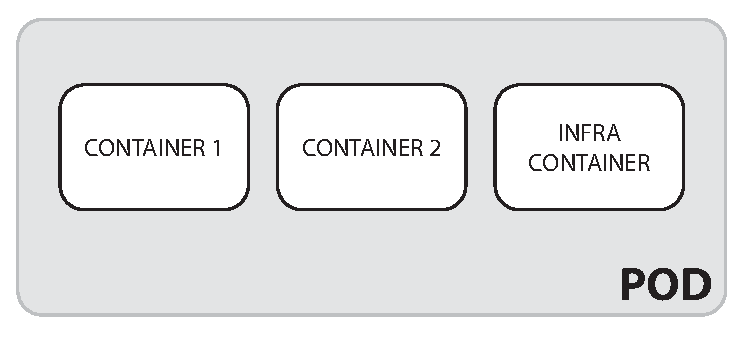
\includegraphics[width=.65\linewidth]{pod.eps}
   \caption{Structure of a pod with two containers created by a user and an infrastructure container}
  \end{figure}


The pod concept in Podman is based on the smallest deployable software units you can create and manage in Kubernetes. 

\textbf{Additional resources:}
\begin{itemize}
 \item \href{https://docs.podman.io/en/latest/markdown/podman-pod.1.html}{Overview} of all  actions available to manage pods
\end{itemize}


\textbf{Read more:}
\begin{mditemize}
 \item \hyperref[podman-overview]{Podman overview}
 \item \hyperref[container-overview]{Containers overview}
\end{mditemize}


\hypertarget{podman-overview}{%
\subsection{Podman overview}\label{podman-overview}}
%\begin{mdblockquote}
 \textit{This section provides basic information on the Pod Manager tool (Podman).}
%\end{mdblockquote}

Podman is an open-source tool designed to create and manage pods and containers. It can be used as a drop-in replacement for docker but has unique features. Podman is:
\begin{mditemize}
 \item \textit{\textbf{daemonless}} - it launches pods and containers as child processes rather than a program running in the background.
\item \textit{\textbf{rootless}} - you don’t need root privileges to create and manage pods and containers.
\item \textit{\textbf{safe}} - while pods and containers don’t have root privileges, they provide a barrier against external attackers.
\item \textit{\textbf{modular}} - it relies on other tools to build and manage container images.
\end{mditemize}

\hypertarget{container-overview}{%
\subsection{Containers overview}\label{container-overview}}
%\begin{mdblockquote}
 \textit{This section provides basic information on container and containers images.}
%\end{mdblockquote}

Containers provide an isolated environment for applications. A typical container consists of application binary, file system, environment settings, and needed libraries. 

Containers are runtime instances of container images, which are executable files designed to be platform-independent and organized in a layered fashion. Images can be downloaded as ready-to-use executables from a registry, a service that stores container images. According to the user's needs, they can be used directly or modified. You also can create your images from scratch.
 

\hypertarget{api-overview}{%
\section{Podman REST API overview}\label{api-overview}}
%\begin{mdblockquote}
 \textit{This section provides basic information on the REST API implemented in  Podman.}
%\end{mdblockquote}

Application programming interface (API) provides a simple method of communication between products or services. Software developers mostly use it to integrate new applications into existing architecture.

Podman REST API is split into two layers:
\begin{mditemize}
\item Compatible with Docker called \mdinlinecode{Compat API}
\item Native API called \mdinlinecode{Libpod API} providing access to additional features not available in Docker, such as pods
\end{mditemize}

New users should use native \mdinlinecode{Libpod API} when starting working with Podman. \mdinlinecode{Compat API} is provided for the current Docker users to help adopt Podman instead of Docker.

\hypertarget{creating-pods-using-rest-api}{%
\section{Creating pods using REST
API}\label{creating-pods-using-rest-api}}
\textit{This procedure demonstrates creating a pod with two containers using native REST API on Fedora Linux. It is based on a typical example of creating a UI application with an associated database.}

\hypertarget{prerequisites}{%
\textbf{Prerequisites}\label{prerequisites}}

\begin{mditemize}
\item
  \mdinlinecode{podman} and \mdinlinecode{curl} packages are installed.
  
\begin{mdcodeblock}
$ sudo dnf install podman curl
\end{mdcodeblock}
  \item Podman manually started as a service with user privileges. 
  
 \begin{mdcodeblock}
$ podman system service -t 0 &
\end{mdcodeblock}
\item Container images \mdinlinecode{wordpress} and \mdinlinecode{mariadb} are downloaded.
\begin{mdblockquote}
 \textbf{Note:}
 You can download container images using \href{https://docs.podman.io/en/latest/markdown/podman-pull.1.html}{the CLI} interface or \href{https://docs.podman.io/en/v3.2.3/_static/api.html#operation/ImagePullLibpod}{REST API}.
\end{mdblockquote}

\end{mditemize}


\hypertarget{procedure}{%
\textbf{Procedure}\label{procedure}}
\begin{mdenumerate}
\setlength\itemsep{1em}
\item
  Create a configuration file for the \mdinlinecode{mariadb} database container named \mdinlinecode{my-pod.conf}.

\begin{mdcodeblock}
{
    "portmappings": [
    {
        "container_port": 80,
        "host_port": 8080
    }
    ],
    "name": "my-pod"
}
\end{mdcodeblock}

\begin{mdblockquote}
 \textbf{Note:} 
 \begin{mditemize}
  \item Configuration file contains only port mapping and a pod name.
  \item There are more fields that can be filled. If not supplied, they receive
  default values.
 \end{mditemize}

  
\end{mdblockquote}

\item
  Create an empty pod by sending \mdinlinecode{POST} request with \mdinlinecode{content-type:application/json} header to the \mdinlinecode{libpod/pods/create} endpoint, with \mdinlinecode{my-pod.conf} as a configuration file.

\begin{minipage}{0.945\textwidth}
\begin{mdcodeblock}
$ curl -XPOST --unix-socket /run/user/${UID}/podman/podman.sock \
    -H content-type:application/json \
    http://d/v3.0.0/libpod/pods/create -d @my-pod.conf
\end{mdcodeblock}
\end{minipage}

\begin{mdblockquote}
\textbf{Note:}
  \begin{mditemize}
  \item
    \mdinlinecode{\$\{UID\}} is the bash variable that returns the current user ID
    \item \mdinlinecode{/run/user/\$\{UID\}/podman/podman.sock} is the socket address of a podman service ran with the user privileges.
  \end{mditemize}
\end{mdblockquote}
 \textbf{Expected output:} JSON structure with pod ID.


\item  Create a configuration for the \mdinlinecode{mariadb} database container named \mdinlinecode{mariadb.conf}.
\begin{mdcodeblock}
{
    "image" : "wordpress",
    "env": {
        "MYSQL_ROOT_PASSWORD": "w0rdpr3ss",
        "MYSQL_DATABASE": "wp",
        "MYSQL_USER" : "wordpress",
        "MYSQL_PASSWORD" : "w0rdpr3ss"
    },
    "restart_policy": "always",
    "pod": "my-pod",
    "name": "mariadb"
}
\end{mdcodeblock}
\begin{mdblockquote}
  \textbf{Note:}

  \begin{mditemize}
  \item
    \mdinlinecode{env} section contains environment variables that will be passed to the container.
  \item
    In the case of a failure, the container will be restarted due to
    \mdinlinecode{restart\_policy} set to \mdinlinecode{always}.
  \end{mditemize}

\end{mdblockquote}
\item  Create a container named \mdinlinecode{mariadb} in the existing \mdinlinecode{my-pod} pod
by sending \mdinlinecode{POST} request to the \mdinlinecode{libpod/containers/create} endpoint, with \mdinlinecode{mariadb.conf} as a configuration file.


\begin{mdcodeblock}
$ curl -XPOST --unix-socket /run/user/${UID}/podman/podman.sock \
    -H content-type:application/json \
    http://d/v3.0.0/libpod/containers/create -d @mariadb.conf
\end{mdcodeblock}
 \textbf{Expected output:} JSON structure with container ID and warnings list.

\item
  Create a configuration file for the \mdinlinecode{wordpress} container named
  \mdinlinecode{wordpress.conf}.

\begin{mdcodeblock}
{
    "image" : "wordpress",
    "env": {
        "WORDPRESS_DB_NAME": "wp",
        "WORDPRESS_DB_USER": "wordpress",
        "WORDPRESS_DB_PASSWORD" : "w0rdpr3ss",
        "WORDPRESS_DB_HOST" : "127.0.0.1"
    },
    "pod": "my-pod",
    "name": "wordpress"
}
\end{mdcodeblock}
\item
Create a container named \mdinlinecode{wordpress} in the existing \mdinlinecode{my-pod} pod
by sending \mdinlinecode{POST} request to the \mdinlinecode{libpod/containers/create} endpoint, with \mdinlinecode{wordpress.conf} as a configuration file.

\begin{mdcodeblock}
$ curl -XPOST --unix-socket /run/user/${UID}/podman/podman.sock \
    -H content-type:application/json \
    http://d/v3.0.0/libpod/containers/create -d @wordpress.conf
    \end{mdcodeblock}
     \textbf{Expected output:} JSON structure with container ID and warnings list.
% \item
%   Optional: Inspect \mdinlinecode{my-pod} to check if \mdinlinecode{wordpress},
%   \mdinlinecode{mariadb} and internal \mdinlinecode{infra} containers are in
%   configured state.

% \begin{mdcodeblock}
% $ curl  --unix-socket /run/user/${UID}/podman/podman.sock \
%     http://d/v3.0.0/libpod/pods/my-pod/json | jq
% ...
% {
%     "Id": "ef494608cee76dcf2e03d79704c5984819fafefec93bbf86c08b165213ce80f2",
%     "Name": "my-pod",
%     "Created": "2022-04-11T22:50:58.066046201+02:00",
%     "State": "Created",
%     ...
%     "NumContainers": 3,
%     "Containers": [
%         {
%             "Id": "8a886dee57899e5eabd2f9c9e9b47c7ee0ba14b7aee12db4872a51f71fad166c",
%             "Name": "mariadb",
%             "State": "configured"
%         },
%         {
%             "Id": "e5a8a346863953560daa53dcbb53db7523debac96cf88481f8bc88e84aaf8141",
%             "Name": "wordpress",
%             "State": "configured"
%         },
%         {
% %             "Id": "e84d75413878516a16df3b96cddefafbdf2f5905f77a33851b274e00a372d406",
%             "Name": "ef494608cee7-infra",
%             "State": "configured"
%         }
%     ]
% }
% \end{mdcodeblock}
\item
  Start \mdinlinecode{my-pod} pod by sending \mdinlinecode{POST} request to the \mdinlinecode{libpod/pods/my-pod/start} endpoint.

\begin{mdcodeblock}
$ curl -XPOST --unix-socket /run/user/${UID}/podman/podman.sock \
    -H content-type:application/json \
    http://d/v3.0.0/libpod/pods/my-pod/start
\end{mdcodeblock}

  \textbf{Expected output:} JSON structure with pod ID and a potential error field.
\item
  Optional: Inspect in your web browser \mdinlinecode{wordpress} application
  running on \mdinlinecode{http://localhost:8080/}
  
  \textbf{Expected output: }
  \begin{figure}[H]
  \centering
   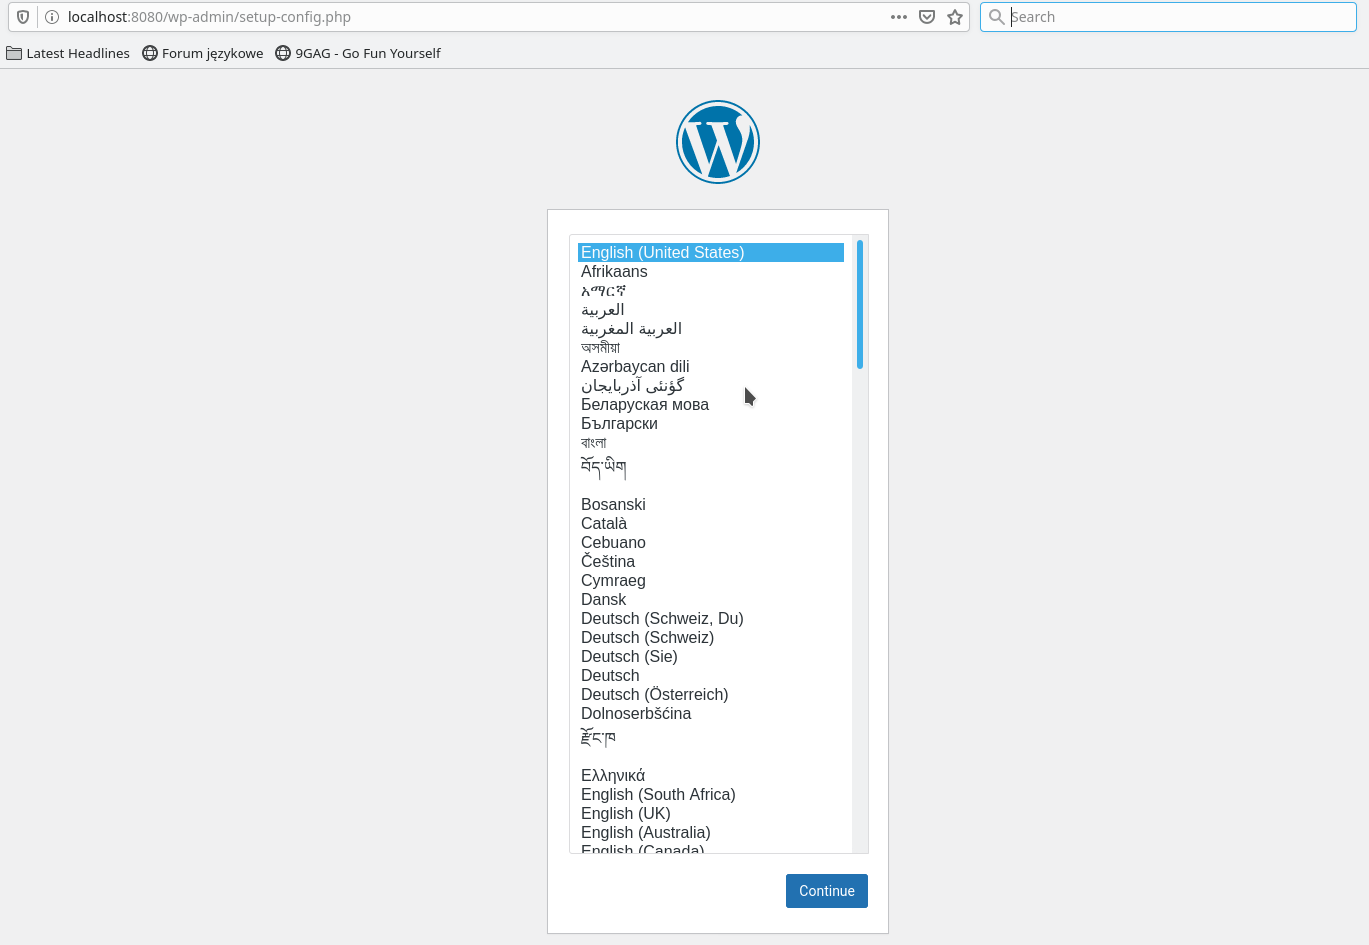
\includegraphics[width=.95\linewidth]{res.png}
   \caption{WordPress running inside a pod}
  \end{figure}

\end{mdenumerate}
\setlength\itemsep{1em}
\hypertarget{additional-resources}{%
\textbf{Additional resources}\label{additional-resources}}

\begin{mditemize}
\item
  \mdinlinecode{podman-pod-create} man page
\item
  Podman API documentation on \href{https://docs.podman.io/en/v3.2.3/_static/api.html#operation/PodCreateLibpod}{creating} and \href{https://docs.podman.io/en/latest/_static/api.html#operation/PodStartLibpod}{starting} a pod
  \item Podman API documentation on \href{https://docs.podman.io/en/latest/_static/api.html#operation/ContainerCreateLibpod}{creating} a container
\end{mditemize}

\hypertarget{getting-pods-using-rest-api}{%
\section{Getting pod information using REST
API}\label{getting-pods-using-rest-api}}
\textit{This procedure demonstrates how to get pod information using native REST API on Fedora Linux.}

\textbf{Prerequisites}

\begin{mditemize}
\item
  \mdinlinecode{podman}, \mdinlinecode{curl}, and \mdinlinecode{jq} packages are installed.
  
\begin{mdcodeblock}
$ sudo dnf install podman curl jq
\end{mdcodeblock}
  \item Podman manually started as a service with user privileges. 
  
 \begin{mdcodeblock}
$ podman system service -t 0 &
\end{mdcodeblock}
\item At least one pod has been created.
\end{mditemize}
\textbf{Procedure}

\begin{mdenumerate}
 \item List processes running inside \mdinlinecode{my-pod} pod by sending \mdinlinecode{GET} request to the \mdinlinecode{libpod/pods/my-pod/top} endpoint.
 \begin{mdcodeblock}
$ curl --unix-socket /run/user/${UID}/podman/podman.sock \
http://d/v3.0.0/libpod/pods/my-pod/top | jq
\end{mdcodeblock}

%    "USER",
%    "PID",
%    "PPID",
%    "%CPU",
%    "ELAPSED",
%    "TTY",
%    "TIME",
%    "COMMAND"

\textbf{Expected output:} JSON structure with running command name and other important information on running processes like \mdinlinecode{PID}, \mdinlinecode{USER} or CPU usage.

\item Display information describing \mdinlinecode{my-pod} pod by sending \mdinlinecode{GET} request to the \mdinlinecode{libpod/pods/my-pod/json} endpoint.

\begin{mdcodeblock}
$ curl --unix-socket /run/user/${UID}/podman/podman.sock \
http://d/v3.0.0/libpod/pods/my-pod/json |jq
\end{mdcodeblock}
\textbf{Expected output:} JSON structure with all the information describing a pod, such as a name, creation timestamp, number of containers, state of containers, and more.
\end{mdenumerate}
\hypertarget{additional-resources}{%
\textbf{Additional resources}\label{additional-resources}}
\begin{mditemize}
\item
  \mdinlinecode{podman-pod-inspect} and \mdinlinecode{podman-pod-top} man pages
\item
  Podman API documentation on \href{https://docs.podman.io/en/latest/_static/api.html#operation/PodTopLibpod}{listing pod processes} and \href{https://docs.podman.io/en/latest/_static/api.html#operation/PodInspectLibpod}{inspecting} a pod

\end{mditemize}


\hypertarget{stopping-pods-using-rest-api}{%
\section{Stopping pods using REST
API}\label{stopping-pods-using-rest-api}}
\textit{This procedure demonstrates how to stop a pod using native REST API on Fedora Linux.}

\textbf{Prerequisites}
\begin{mditemize}
\item
  \mdinlinecode{podman} and \mdinlinecode{curl} packages are installed.
  
\begin{mdcodeblock}
$ sudo dnf install podman curl
\end{mdcodeblock}
  \item Podman manually started as a service with user privileges. 
  
 \begin{mdcodeblock}
$ podman system service -t 0 &
\end{mdcodeblock}
\item At least one pod has been created.
\end{mditemize}
\textbf{Procedure}
\begin{mdenumerate}
\setlength\itemsep{1em}

 \item Stop \mdinlinecode{my-pod} pod using REST API by sending \mdinlinecode{POST} request to the \mdinlinecode{libpod/pods/my-pod/stop} endpoint.
 \begin{mdcodeblock}
$ curl -XPOST --unix-socket /run/user/${UID}/podman/podman.sock \
-H content-type:application/json \
http://d/v3.0.0/libpod/pods/my-pod/stop
\end{mdcodeblock}
\textbf{Expected output:} JSON structure with pod ID and a potential error field.
\item Optional: You can remove stopped \mdinlinecode{my-pod} pod using REST API if no longer needed. 
 \begin{mdcodeblock}
$ curl -XDELETE --unix-socket /run/user/${UID}/podman/podman.sock \
-H content-type:application/json \
http://d/v3.0.0/libpod/pods/my-pod 
\end{mdcodeblock}
\textbf{Expected output:} JSON structure with pod ID and a potential error field.
\end{mdenumerate}
\hypertarget{additional-resources}{%
\textbf{Additional resources}\label{additional-resources}}
\begin{mditemize}
\item
  \mdinlinecode{podman-pod-stop} and \mdinlinecode{podman-pod-rm} man pages
\item
  Podman API documentation on \href{https://docs.podman.io/en/latest/_static/api.html#operation/PodStopLibpod}{stopping} and \href{https://docs.podman.io/en/latest/_static/api.html#operation/PodDeleteLibpod}{removing} a pod

\end{mditemize}


\end{document}
